\section{Analysis}
\subsection{Related work}




\subsection{Wayfinding}
In the paper Wayfinding (insert reference) which is a DTU project in collaboration with Dalux, the goal was to do a pathfinding for a worker in a building. This is similar to what will be done in this thesis and therefore a lot of the same groundwork is done. The data set is also the same, which makes it easy to translate the results and compare. Even though there was no access to the source code they used to generate their algorithms the report gave good inspiration to what should be done and it also worked as a guide for me to get started. I will be using this report as a reference throughout this thesis.


\subsection{Spot}
%Hvad er cad modeller og robotten.
%Giv en kontekst.
%Hvorfor er vi interesseret i at løse problemet.
The Spot robot is produced by Boston Dynamics and is their first commercially available robot currently being sold for a minimum of 74.500 dollars \cite{spot}. The robot is a quadruped and resembles a 'dog'. The robot can be controlled with a tablet controller, but it can also be programmed to do autonomous tasks. The robot has its own Python SDK. The purpose of the robot is according to their own website: "Spot Explorer is designed for developers eager to explore how flexible mobile robots can be adapted for tasks ranging from industrial inspection to entertainment."\cite{spot}

Industrial inspection is precisely what it will be used for in this project. Although this project does not work with the SPOT robot directly the project does take into consideration it's dimensions and capabilities. 
The actual programming of the robot to walk the path programmed in this project, will be a part of future works of this project. Explained further under Future works section.

One of the SPOT robot's more useful properties is obstacle avoidance. Say we tell the robot to go from a point x to another point y - either by its controller or by a programmed path - if there is an object that blocks the straight line traversal between a point x and point y the robot will be able to detect this object and move around it. 
This is a useful feature because it lets the user give the robot a general path without having to worry about it bumping into   objects that would stand it its way. 
The robot can also walk up stairs which will also be interesting for future development of this project, allowing it not only to walk around one floor but multiple floors.




Include picture of SPOT.
\begin{figure}[H]
    \centering
    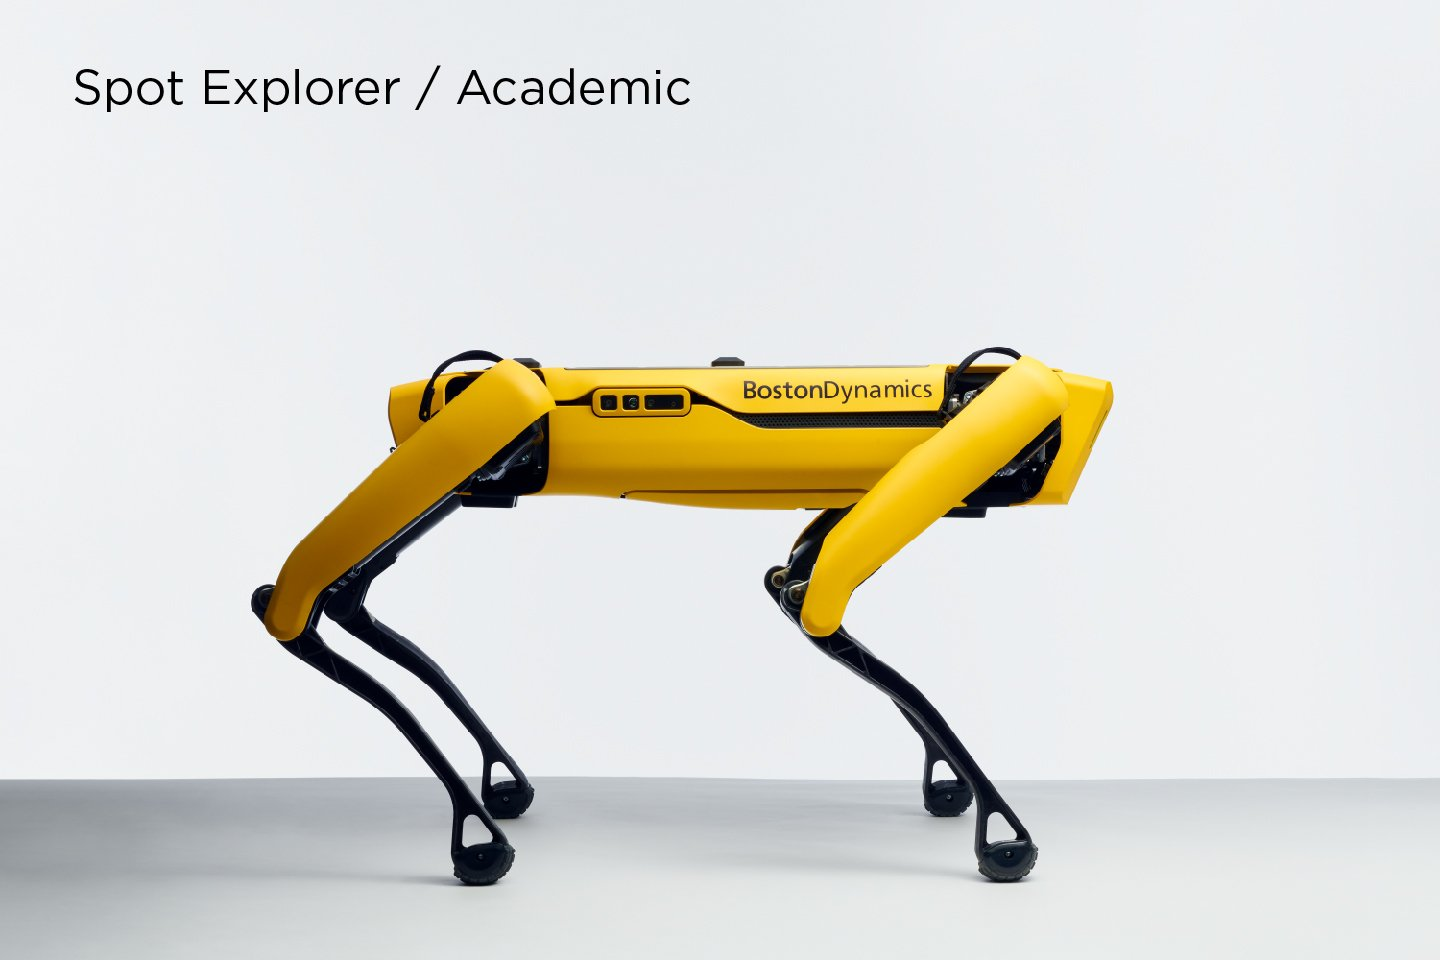
\includegraphics[width=1\textwidth]{fig/Spot Explorer-1.jpeg}
    \label{}
    \caption[The SPOT robot]{Weird floor plan~\cite{spot_robot}}
\end{figure}


\begin{itemize}
    \item Write about Spot and how it is a useful robot for this thesis
    \item How does the robot look and its dimensions.
    \item A little backstory on Spot, who made the robot, and for which purposes
    \item Write about different platforms for programming Spot, python API vs ROS.
\end{itemize}


\subsection{Dataset}

The dataset consists of html code of the room coordinates and the door coordinates in the format of the file is IFC (Industry Foundation Classes). [insert reference: https://fileinfo.com/extension/ifc]
[Insert picture of data]
The coordinates are given in a polygonal triangle structure. This means that the floor plan is drawn from these coordinates by a mesh of triangle polygons. Each room from in the floor plan consists of its own tree branch, which makes it easy to include or exclude rooms in the floor plan.
Describing rooms and floor plans with triangle forming coordinates is a common way and makes sense for many reasons.
(Insert article reference that describes this way of plotting rooms)
(Insert picture of floor plan with triangles).
\\
The door coordinates also consists of the set of 3 coordinates with a x,y and z coordinate. Where the z coordinate says how tall the door is. 
\\
BIM models is also available for use, but will not necessarily be used since we start by modelling in 2D.
(Describe BIM models)
\begin{itemize}
    \item Write the format of the code
    \item Triangulation of the coordinates makes up the room
    \item Write about door information
\end{itemize}

\subsection{Graph Theory}
As explained in the objective section\ref{Objective} of the introduction a big part of this project relies on the use of graphs, and graph theory plays a big role in this project. 
The program is essentially representing the building using two graphs, where one is a subgraph of the other. 
For the first graph the building is discretized and sampled in a grid. Each grid point is in this graph represented by a node. This will be called the "grid"-graph.
For the second graph one can think of the building as a graph with each room represented as a node. This is called the "room"-graph.
In the following sections the relevant graph theory will be explained, which will form a basis for the Travelling salesman algorithm used to solve the pathfinding problem.

- Explain other uses of Graphs (electrical networks).
- Explain the background of graph theory, why is it interesting, and why did I choose it in the program.

\subsubsection{What are graphs?}
A graph essentially consists of nodes and edges.
[Insert graph picture]
[Insert formula for graphs (G(n,e))]
A graph can be directed or undirected. With a directed graph the edge between two nodes represent a one way connection, the edge is thereby "directed" from one node to another. In an undirected graph there is no general direction meaning you can go from node a to node b and from node b to node a. In this project the program works with undirected graphs since if there is a connection between two rooms it is assumed that the robot can walk from room a to room b the same way it can walk from room b to room a, and the cost of the walk will also be identical. \cite{bondy1976graph}
- Write about edge weights

\subsubsection{Connectivity}
The approximate solution to the traveling salesman problem used in this program has a prerequisite that the graph used is fully connected also defined as complete.  
Connectivity is a measure of how connected the nodes of the graph are. A minimal connected graph is a graph that if one of the edges is removed the graph will become disconnected. A fully connected or complete graph is a graph where every node has a edge to every other node in the graph. [insert picture of the two examples.] \cite{bondy1976graph}


\subsubsection{Minimum spanning tree}
Another notion used to solve Traveling salesman problem is the minimum spanning tree (MST). The idea behind minimum spanning tree is to find the minimal connected graph with the minimum summed edge weights. For a given graph there can be \cite{hej} multiple minimum spanning trees since different trees can have the same minimum summed edge weights.\cite{cormen2009introduction}



Different algorithms to find the minimum spanning tree. In this program the minimum spanning tree is found using the build in function in the networkx library. This function uses Kruskals algorithm to find the minimum spanning tree. chapter[23.2]\cite{cormen2009introduction}


- Explain that in this program the minimum spanning tree makes up the room graph. and for that to work we need to find the shortest distance between each room node that will make up the edge between the room nodes.

\subsubsection{Kruskals algorithm}
%chapter[23.2]\cite{cormen2009algo}
%[reference:https://cp-algorithms.com/graph/mst_kruskal.html]
%[reference2: https://www.cs.cmu.edu/afs/cs/academic/class/15451-s04/www/Lectures/minimumSpanningTrees.pdf, dette er bogen som du selv også har]

\subsubsection{Shortest path problem}
Before finding the minimum spanning tree Another important thing to do to find the minimum distance between two nodes in a graph.
In this program the A star algorithm is used from the networkx library. The A star is proved to be optimal and faster than its predecessors. It builds upon dijkstras algorithm.

- Explain the A star algorithm



\subsection{Traveling salesman problem}

- Explain about the traveling salesman problem, background and history
- Usefulness in the program
- Alternatives?
- It is a NP hard problem
- Approximate solutions, A section of the 2-OPT algorithm and how it uses Minimum Spanning Tree and a DFS traversal. You can talk about alternative algorithms and their pros and cons. \cite{flood1956traveling}


\subsubsection{Hamiltonian cycle}
- Explain what they are 

\begin{itemize}
    \item \sout{Why we use graph theory}
    \item \sout{What are graphs?}
    \item \sout{Undirected graphs}
    \item \sout{Connectivity, which is important for the Traveling salesman problem}
    \item \sout{Minimum spanning tree}
    \item \sout{Shortest path problem}
    \item \sout{Hamiltonian cycle}
    \item \sout{Travelling salesman problem}
\end{itemize}



\subsection{Spatial Data structures}
- What are they and Why do we need spatial datastructures
- Explain different forms for spatial datastructures
- Explain the Rtree in depth
- Explain the Rtree library used, perhaps.

\subsection{Distance field or visibility graph}
- What is it and why is it useful
- Explain alternatives

\subsection{Optimal placement of nodes}
- Explain K means
- Explain Convex decomposition





















%-----------------------------------------------%
\begin{comment}
\subsection{Grid vs polygonal}
\subsubsection{Unity vs python}
The problem with unity was that it was difficult to import floorplans in a good way.

Talk about how you could use the grid version or the polygonal version. Spent a good amount of effort here.

\subsection{Which platform to use}
\begin{itemize}
    \item Write about which platform to use. The pros and cons of each. Ros vs Unity vs Python.
\end{itemize}








\subsection{Dijkstra's algorithm}
Dijkstra's algorithm is an algorithm to find the shortest path between two nodes in graph. The way it works is by first having a source node or initial node. The distances to all other nodes will be initialized to infinity since the distances are unknown for now. Then the algorithm will look at the neighbour nodes of the source node. It will evaluate the distance to each of the nodes. The distances of the nodes will then be updated in the table of distances, since it is no longer infinity. With done the start node has been visited and will no longer be visited. The next node in the algorithm to evaluate will be the node with the shortest distance to the start node. The neighbours to this node will now be evaluated and again the distance table will be updated. This pattern will keep repeating until all nodes have been evaluated. 

\subsection{A*}
A

\subsection{How to get around the building}
The way to get around the building is using visibility graph. Here you make a node on each portruding corner and also on the doors. This way a path between all nodes can be constructed, this is called a visibility graph.
(reference the master thesis).

\subsubsection{Convex decomposition}
In the report written by nikolaj and co. The way they solved the general pathfinding problem through the building was using Convex Decomposition. The idea in convex decomposition is to split non convex polygons - in this case the polygons represent the rooms of the floor - into convex subparts. Each convex subroom will then be assigned a node. A room is non convex if a corner of the room has an angle of more than 180 degrees. In these cases we get scenarious where 2 nodes in the same room are not necessarily connected by a straight path [insert sketch]. A convex room on the other hand has no corners of more than 180 degrees and therefore ensures that any 2 nodes in room is connected by a straight path. 
When a room is divided into its convex subparts a node is placed in the intersection of these two rooms and connection is thereby ensured between all areas in the original room.
Doing this convex decomposition of the rooms therefore makes the use of corner nodes superfluous since role of the corner nodes was to make this connection between the different areas of the non convex rooms.

Convex decomposition has a limitation when it comes to obstacles - that are visible from the graph i.e pillars - it has no good way to deal with these. This is the same with the portruding corner node approach. Neither of these two have good ways to deal with obstacles or narrow paths.

\subsubsection{The challenge of obstacles}
What to do with these obstacles like pillars.


\subsection{How to get from room to room/around the building in an appropriate way?}
Do we want the shortest route?
Do we want the route


\subsection{The precise objective of the project}
When doing a project such as this one where there are many alternative solutions with each of their pros and cons, it is important to have a very clear and precise objective such that you know what features are important to look for and which are not important. For example is it necessary that the robot finds the optimal path or is it just a bonus? The important thing is not that the robot finds the optimal path necessarily but rather that it gets to walk around the entire building (or as much as possible) in one charge - that is 90 minutes. More precisely put the objective is for the robot to do point scans of as much of the building as possible.

The reason optimality is not necessary is that we don't really pay the robot by the hour as we would do if a human were to do the walk.
Whether it takes the robot 30 minutes or 50 minutes to walk around the building is not really important. Route stability is more important than route optimality in this case.
This knowledge and realisation will help us in deciding which algorithm and approach to use when doing the pathfinding. It means that we would rather have that the robot finds a way to get around the building with certainty rather than it having to walk an optimal route, that for different reasons may not be realisble in reality.


But how do we know if the robot can do the walk in 90 minutes? 
This would have to be calculated somehow?

So the goal of the project is to make a robot walk around one floor of a building in such a way that it gets.

Is optimal node placements necessary ? 

Is performance important ? Not really, since it is not in real time. Unless it takes many days for the program to run.



\subsection{Dimensions of robot/ collision detection}
\begin{itemize}
    \item Write about how to incorporate the dimensions of the robot in your simulation
\end{itemize}


\subsubsection{Distance field vs distance route}
The dimensions of the robot is mostly needed to make sure that the robot does not bump into walls or other objects. And also to make sure that a path that is deemed traversable is not in reality too narrow for the robot to pass through.
So far the robot has been modeled by a point, it is now time to include a radius to that point which will represent the robots dimensions.

There are mainly 3 concerns for the robot when it wants to traverse the floorplan now. One is the concern of too narrow paths. The other is the concern of obstacles that are seen from the floorplan i.e pillars. And the third are obstacles not seen from the floorplan, maybe a chair or a table etc.



There are multiple ways to go about the challenge of incorporating the dimensions of the robot in the simulation. 
One way is to discretize the entire map and for each cell find the distance to the nearest wall. If the distance from the wall to the cell is smaller than the radius of the robot, the cell will be deemed not traversable since this means that the robot will hit the wall. If the distance to the wall is larger than the radius the cell is traversable. What we get by doing this is a boolean distance field. Where we have nodes that are traversable and nodes that aren't.
The issue with this approach is that it is not very scalable to bigger buildings. More on this is written in chapter 10.
The good thing about this approach is that it is easy and a straightforward way to tell the robot which places it is allowed to traverse and which are not. It can not go wrong with this approach. 
It is also fast to look up because you have done the preprocessing before hand.
Another pro of this approach is that it will be beneficial when we later want to find optimal node placements in the rooms we are visiting.

The other way is to discretize the route. This is a bit more complicated implementation but will be rewarded by its scalability to bigger buildings. 
The idea here is to only discretize the route that the robot will walk instead of discretizing the entire map. 
Along the route  the robot will check if it is near a wall using a distance function. The interval here can be dynamic e.g if the distance to the nearest wall is 5 meters and the radius of the robot is 1 meter it can walk for 4 meter without hitting a wall.
This means that between 2 nodes - a start and an end node - a lot more nodes will be placed. The robot will go to a node find the distance to the nearest wall and then check walk in a straight line towards the node it is seeking the same amount as the distance to the nearest wall minus the radius. Then it will check again to see what the distance to the nearest wall is and repeat the process. It is important that the room/end nodes are a certain radius away from the walls to begin with. 

One way to go about this is to check the distance to all the walls for every node. This does not scale very well when the number of walls increases. 
Another way is to have a certain datastructure that takes all the walls and find the nearest quickly.

One other problem with discretizing the route is that a large percentage of the time the obstacle between 2 room nodes are walls and this means that this A star algoritm will often fail, since the only way to walk through walls are using the doors. 

A third way is to follow the same scheme as has been done so far and only rely on corner nodes and door nodes to go from node to node. This should in theory work and should only not work when we have a straight path that is too narrow. In these cases which will be very rare what will happen is that the robot wont be able to walk through it and we will tell it that it should do the tsp solution again and make the connection between these two nodes not traversable.



So how is convex decomposition related to the dimensions of the robot? Well doing convex decomposition by itself does not ensure that all nodes placed on the floorplan are in accordance with the requirements needed to allow for the dimension of the robot. This technique would have to be combined with a distance measure to the nearest wall being larger than the radius of the robot.


\subsubsection{Random placements of nodes}
I will have to think about this mehtod.
In this method the idea

\subsubsection{A star discrete route}
This is the second argument in this area.


\subsection{Data structure for the walls}
Explain the purpose of space partitioning algorithms

\subsubsection{Binary space partitioning}
Binary space partitioning trees is a datastructure used to partition polygons in space. One of its big uses are in computer graphics where it is used as a solution to the issue of Visual surface determination. [insert reference: https://twobithistory.org/2019/11/06/doom-bsp.html]
The renderer of a computer game has to figure out which objects can be seen and not seen from the vievpoint of the player.

Compared to raytracing which is an image first renderer BSP is an object first renderer. This means that rather than tracing each pixel in an image like raytracing does, BSP traces each object in the scene and is therefore more cost effective.

BSP trees are useful when wanting to display the viewpoint of an agent. Since it splits the areas in lines such that there are polygons behind and in front of each line. This is not really what we are looking for in this project. For us i doesn't matter whether the closest wall is directy in front of the robot or directly behind it since this doesn't influence whether it will hit the wall. Or maybe it is only necessary to look at walls straight ahead of you?

BSP is used in collision detecting in robotics. [ref: https://www.wikiwand.com/en/Binary_space_partitioning]
A disadvantage of binary space partitioning is that generating a BSP tree can be time-consuming.Typically, it is therefore performed once on static geometry, as a pre-calculation step, prior to rendering or other realtime operations on a scene. It is an expensive pre process. 

It may not be useful here since we are not working on real time applications.





\subsubsection{KDtrees}
Hvorfor du vælger kd TRees i forhold til BSP trees.
The idea here is to cut the space into halves.
binary search tree with multiple values.
Still a logarithm search in terms of number of nodes in the tree.
You pick a random dimension.
You find the median.
You split the data. 
Pick another dimension. etc.

Usefull algorithm to find nearest neighbour.


The idea behind this structure is to take the center point of each line and partition it into 1 of 4 or 16 corners. Lets start with 4 for simplicity. For each line center we check if its x value is larger or smaller than the grid center x value. If it is larger this means that it will be placed on the right hand side of the map. We then check the y value and do the same. IF it is larger than the center y we place it on the upper part of the map and if it is smaller we place it in the lower part of the map. We have now partitioned the walls into one of 4 sections. We can partion it further if we wish so. A more stable approach is to take each of the points that the line consists of and do the partioning for each point. In this case the line can be part of multiple areas of the map. This is more stable since we can have scenarious of big walls that strectch multiple areas of the map and the grid point could be very close to one of the edge points of the line but not very close to the center of the line.
For each grid point we then check where in the map it is partioned. 

A scenario where this algorithm could fail is when it is close on the edge between two adjacent areas. In this case there could be a scenario where it is closer to a wall on the adjacent area than any of the walls in the area that it is in.
This can be made a non issue by making sure that the point is not less than the radius of the robot away from the intersection between the two areas. If this is the case it doesn't matter if it is closer to a wall on an adjacent area because it will still conform to the dimensions of the robot. 



















\subsection{Optimal placement of nodes}
\begin{itemize}
    \item Write about scenic route vs discrete points.
    \item Write about SLAM
    \item optimal placement of nodes
\end{itemize}

\subsubsection{Simultanous location and mapping}
As the name indicates SLAM is about localizing your robot in the map while you also do the mapping part. The way this is done is by using sensors such as a lidar - it could also be other types of sensors. Then there are some other steps in the process. Since inn this case the mapping has already been done it doesn't really make sense to do the SLAM. It might be a good idea to find a way for the robot to localize itself, without need to do the mapping.




\subsubsection{ROS}
ROS had a pretty smart technique of importing floorplans

\subsubsection{Python API}



\subsection{Future work}
\begin{itemize}
    \item A section about stairs
\end{itemize}

\end{comment}
